\section{MOS Operationsverstärker}
'Operationsverstärker' ist ein \textbf{Sammelbegriff} für Differenzverstärker mit sehr grosser Verstärkung.

\smallskip

Der \textbf{ideale} Operationsverstärker erfüllt zwei Bedingungen:
\begin{itemize}
    \item Es fliesst kein Strom in die Eingänge
    \item Die Spannungsdifferenz zwischen den Eingängen ist null
\end{itemize}

\medskip

Man unterscheidet dabei zwischen \textbf{zwei Arten} von Operationsverstärkern:
\begin{description}
    \item[OTA:] Der Transimpedanz-Operationsverstärker hat eine Spannung am Eingang und liefert am Ausgang einen Strom
    \item[OpAmp:] Der OpAmp verstärkt die Eingangsspannung zu einer Ausgangsspannung 
\end{description}

\begin{ctabular}{|c|c||c|c|}
    \hline
    \multicolumn{2}{|c||}{\textbf{OTA}}                 & \multicolumn{2}{c|}{\textbf{OpAmp}}           \\
    \hline
    $Z_{\rm in} \to \infty$ & $Z_{\rm out} \to \infty$  & $Z_{\rm in} \to \infty$ & $Z_{\rm out} \to 0$ \\
    \hline
\end{ctabular}

\vspace{-0.2cm}


\subsection{Struktur}

\begin{center}
    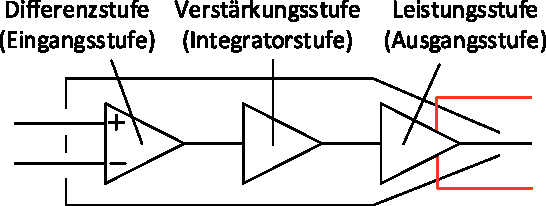
\includegraphics[width=0.65\columnwidth]{images/09_OpAmp_struktur.pdf}
\end{center}

\begin{outline}
    \1 \textbf{Differenzstufe}
        \2 Bildet die Differenz zwischen $V+$ und $V-$ und verstärkt diese
    \1 \textbf{Verstärkerstufe}
        \2 Erhöht die Verstärkung und bestimmt meist die Bandbreite
    \1 \textbf{Leistungsstufe}
        \2 Wandelt die hohe Impedanz in eine kleine Ausgangsimpedanz
            \textrightarrow\ \textbf{fehlt beim OTA}
\end{outline}


% \subsubsection{Differenzstufe}
% Bildet die Differenz zwischen $V+$ und $V-$ und verstärkt Differenzstufe

% \subsubsection{Verstärkerstufe}
% Erhöht die Verstärkung und bestimmt meist die Bandbreite.

% \subsubsection{Leistungsstufe}
% Wandelt die hohe Impedanz in eine kleine Ausgangsimpedanz.
% Diese Stufe fehlt beim OTA.


\subsection{Differenzstufe -- Grosssignalanalyse}

\subsubsection{Strong Inversion}

\begin{minipage}[t]{0.48\columnwidth}
    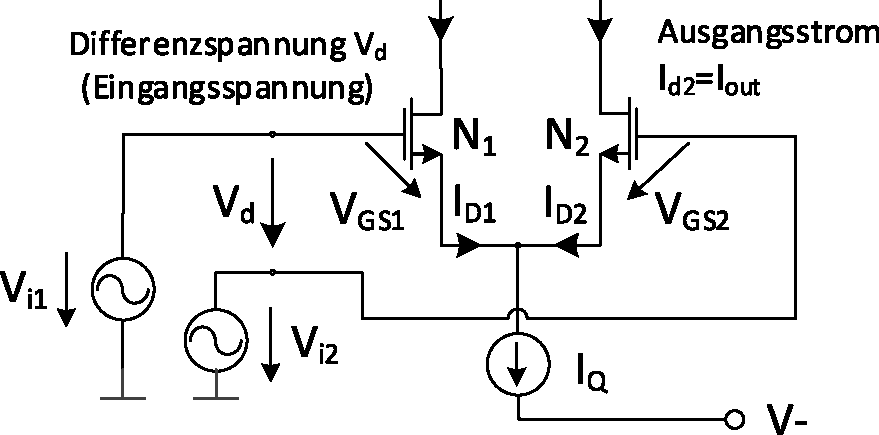
\includegraphics[width=\columnwidth, align=t]{images/09_differenzstufe_grosssignalanalyse.pdf}
\end{minipage}
\hfill
\begin{minipage}[t]{0.48\columnwidth}
    \begin{align*}
        \text{Sättigung:} \quad     I_\text{D}  &= \frac{\mu C_\text{ox}}{2} \frac{W}{L} (V_\text{GS} - V_\text{T})^2    \\
        \text{Konten:} \quad        I_\text{Q}  &= I_\text{D1} + I_\text{D2} 
    \end{align*}
\end{minipage}

\[
    \frac{I_\text{D}}{I_\text{Q}} = f(V_d) = f(V_{i1} - V_{i2}) = \frac{1}{2} + \frac{1}{2} \sqrt{\frac{\left(\mu C_\text{ox} \frac{W}{L}\right) \cdot V_\text{d}^2}{I_\text{Q}} - \frac{\left(\mu C_\text{ox} \frac{W}{L}\right)^2 \cdot V_\text{d}^4}{4 I_\text{Q}}}
\]


%TODO: [Flurin] Kennlinie aus V10S9
%CHECK: [Simi] @Flurin: There it is... Eventuell ist es aber besser, wdie 3 Bereiche formelmässig darzustellen und die Grafik wegzulassen...?
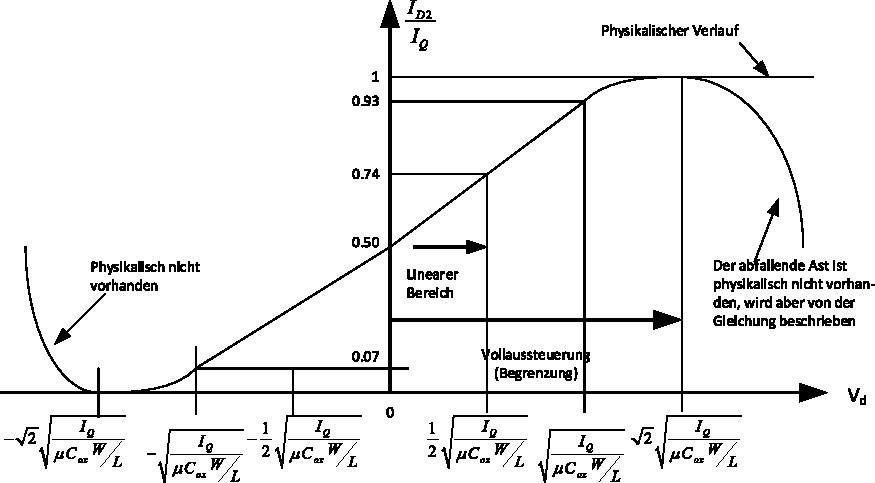
\includegraphics[width=\columnwidth, align=t]{images/09_differenzstufe_grosssignalanalyse_strong_inv.pdf}


\subsubsection{Weak Inversion}
\[
    I_\text{D} = \frac{W}{L} I_\text{M}' e^\frac{V_\text{GS}-V_\text{M}}{n_\text{M} V_\text{temp}}
\]

%TODO: Evtl. Formel ohne vereinfach tanh(x) = x (nicht in den Slides)

Für Kleine $V_\text{d}$:
\[
    \frac{I_\text{D}}{I_\text{Q}} \approx \frac{1}{2} \left(1+\frac{V_\text{d}}{2 n_\text{M} V_\text{temp}}\right)
\]


\paragraph{Conclusion}
Die Verstärkung ist im grossen und ganzen unabhängig von der Eingangsspannung und so vom Arbeitspunkt, der durch die Eingangsspannungen gegeben ist.

\subsection{Differenzstufe -- Kleinsignalanalyse}

\paragraph{Ohne Stromspiegel}
% TODO: Evtl. Schema und Ersatzschaltbild aus V10S11
\[
    g_{md} = -\frac{g_m}{2}
\]

\paragraph{Mit Stromspiegel}
% TODO: Evtl. Schema und Ersatzschaltbild aus V10S11
\[
    g_{md} = -g_m
\]

% TODO: Folien V10S12 (sorry, habe nicht zugehört :( )

\subsubsection{Verstärkung}
% TODO: Jeweilige Schemas einfügen

\paragraph{Widerstandslast}

\[
    a \approx \frac{g_m (R_D \parallel R_{L\text{, ext}})}{2}
\]

\paragraph{Stromquellenlast}

\[
    a \approx \frac{ (R{L\text{, ext}} \parallel r_{DS2} \parallel r_{QL})}{2}
\]

\paragraph{Stromspiegellast}

\[
    a \approx g_m \left(\frac{1}{g_{0, N2}} \Biggm\Vert \frac{1}{g_{0, N2}} \Biggm\Vert R_{L\text{, ext}}\right)
\]

\paragraph{Grenzwertbetrachtungen}
\resizebox{\columnwidth}{!}{
    \begin{tabular}{|l|l|l|}
        \hline
        Betriebsbereich & Grenzwert der Spannungsverstärkung & Grössere Verstärkung bei \\
        \hline
        Starke Inversion & $\displaystyle \abs{a_{\text{max}}} = 2 V_e \sqrt{\frac{\mu C_\text{ox} \frac{W}{L}}{I_Q}} \approx 2 a_e \sqrt{\frac{\mu C_\text{ox} L W}{I_Q}}$ & Ruhestrom $\downarrow$, Fläche $\uparrow$, (Early-Spannung $\uparrow$) \\
        \hline
        Schwache Inversion & $\abs{a_{\text{max}}} = \frac{V_E}{n_M V_\text{temp}} \approx \frac{a_E L}{n_M V_\text{temp}}$ & (Early-Spannung $\uparrow$) \\
        \hline
    \end{tabular}
}
\medskip%

Diese Formeln sollten nicht zur Verstärkungsberechnung verwenden -- sie dienen lediglich zur Darstellung der Bezüge verschiedener Parameter.
% TODO: Evtl mehr Formeln / Bedingungen aus V10S14?


